%-----------------------------------------------------------------------------
%   MPLR Project Report - Fingerprint Spoofing Detection
%   Author : Nicola Ciancia
%
%   The source is pure ASCII (every Unicode-looking symbol is typeset via
%   LaTeX math commands), so the document compiles with any of the three
%   mainstream engines:
%       pdflatex REPORT.tex
%       pdflatex REPORT.tex     % second pass for TOC / cross-refs
%   or equivalently   xelatex / lualatex   (no other change needed).
%-----------------------------------------------------------------------------

\documentclass[11pt,a4paper]{article}

\usepackage[a4paper,margin=2.2cm]{geometry}
\usepackage[utf8]{inputenc}
\usepackage[T1]{fontenc}
\usepackage{lmodern}
\usepackage[english]{babel}

\usepackage{amsmath}
\usepackage{amssymb}
\usepackage{amsfonts}
\usepackage{mathtools}
\usepackage{bm}

\usepackage{graphicx}
\usepackage{booktabs}
\usepackage{longtable}
\usepackage{tabularx}
\usepackage{array}
\usepackage{multirow}
% Left-aligned (ragged-right) flexible-width column for tabularx.  Plain X
% justifies, which combined with long \texttt{} strings produces nasty
% overlaps; L avoids it without changing the column-width algorithm.
\newcolumntype{L}{>{\raggedright\arraybackslash}X}

\usepackage{xcolor}
\usepackage{microtype}
\usepackage{caption}
\usepackage{float}
\usepackage{enumitem}
\usepackage{fancyvrb}
\usepackage{seqsplit}              % \seqsplit{...} for breakable monospaced strings
\usepackage[htt]{hyphenat}         % allow hyphenation inside \texttt{}

\usepackage[hidelinks]{hyperref}
\hypersetup{
    colorlinks  = true,
    linkcolor   = blue!50!black,
    urlcolor    = blue!50!black,
    citecolor   = green!50!black,
    pdftitle    = {Project Report - Fingerprint Spoofing Detection},
    pdfauthor   = {Nicola Ciancia},
    pdfsubject  = {Machine Learning and Pattern Recognition},
    bookmarksnumbered = true
}

\graphicspath{{images/}}

\setlist[itemize]{leftmargin=*, itemsep=2pt}
\setlist[enumerate]{leftmargin=*, itemsep=2pt}

\captionsetup{font=small,labelfont=bf,skip=4pt}
\setlength{\parskip}{4pt plus 1pt}
\setlength{\parindent}{0pt}

% Line-breaking: be lenient so long \texttt{} strings (filenames with
% underscores, full function signatures, etc.) do not overflow into the
% margin. \sloppy lets LaTeX prefer ugly spacing over overfull boxes;
% \emergencystretch gives an extra elastic budget for the worst cases.
\sloppy
\emergencystretch=3em
\hbadness=10000   % silence the badness=10000 warnings produced by \sloppy

% Shorthand commands
\newcommand{\actDCF}{\textrm{actDCF}}
\newcommand{\minDCF}{\textrm{minDCF}}
\newcommand{\DCF}{\textrm{DCF}}
\newcommand{\llr}{\textrm{llr}}
% Breakable monospaced text - use this in table cells or whenever a long
% identifier (path, function signature) must wrap.  Internally splits at
% every character via \seqsplit so any width is acceptable.
\newcommand{\code}[1]{\texttt{\seqsplit{#1}}}

\title{\textbf{Project Report}\\[0.3em]
       \Large Fingerprint Spoofing Detection}
\author{Nicola Ciancia\\[0.2em]
        \small\textit{Machine Learning and Pattern Recognition}}
\date{May 20, 2026}

\begin{document}
\maketitle

\begin{abstract}
\noindent
This report describes the implementation and evaluation of a complete
pipeline of binary classifiers on the \emph{fingerprint spoofing
detection} dataset (6000 samples, 6 features, labels \{0=fake,
1=genuine\}). We compare generative Gaussian models (MVG, Naive Bayes,
Tied), discriminative models (standard / prior-weighted / quadratic
Logistic Regression, linear / poly / RBF SVM) and mixture models
(GMM full / diagonal / tied). Results are evaluated with \emph{minDCF}
and \emph{actDCF} for the target application $\tilde{\pi}=0.1,\,
C_{fn}=C_{fp}=1$. The minDCF-winning model (0.1495 full / 0.1324
diagonal) is the \textbf{GMM} with 1 component for the fake class and
16 for the genuine class, consistent with the multi-cluster structure
of features 5 and 6 revealed in the exploratory phase.
\end{abstract}

\tableofcontents
\newpage

%-----------------------------------------------------------------------------
\section{Executive summary}\label{sec:exec}
%-----------------------------------------------------------------------------

The project task is a \textbf{binary classification} problem for
fingerprint spoofing detection. The dataset
(\texttt{Project/data/trainData.txt}) contains 6000 samples, each
described by 6 real-valued features, with binary labels:
\begin{itemize}
\item \textbf{0 = fake} (impostor, counterfeit)
\item \textbf{1 = genuine} (legitimate user)
\end{itemize}

The dataset is nearly balanced (2990 fake / 3010 genuine).

The whole project pipeline uses a \textbf{deterministic
$\tfrac{2}{3}$ vs $\tfrac{1}{3}$ split} with \texttt{seed=0}
(\texttt{utils/data\_utils.py::split\_db\_2to1}), yielding:
\begin{itemize}
\item DTR / LTR: 4000 model-training samples (empirical $\pi_1 \approx 0.5005$)
\item DVAL / LVAL: 2000 validation samples
\end{itemize}

The \textbf{target application}, fixed from Lab 6 onwards, is
$\tilde{\pi}=0.1$, $C_{fn}=C_{fp}=1$ (the ``many impostors'' case:
accepting a fake is penalized more strongly).

\paragraph{Summary of best results on DVAL ($\tilde{\pi}=0.1$).}

\begin{table}[H]
\centering
\begin{tabular}{llrr}
\toprule
Family                  & Best model                                   & minDCF & actDCF \\
\midrule
Generative Gaussian     & MVG (all features)                           & 0.2629 & 0.3051 \\
Logistic Regression     & Quadratic LR ($\lambda \approx 3.2\cdot 10^{-2}$) & \textbf{0.2436} & 0.4972 \\
SVM                     & RBF SVM ($\gamma=e^{-2}$, $C=32$)             & \textbf{0.1725} & 0.4226 \\
GMM                     & Full-cov GMM ($K_0=1$, $K_1=16$)             & \textbf{0.1495} & 0.2055 \\
\bottomrule
\end{tabular}
\end{table}

The minDCF-winning model is the \textbf{full-covariance GMM} with 1
component for the fake class and 16 for the genuine class. This result
is perfectly consistent with the exploratory structure of the dataset
(cf.\ \S\ref{sec:lab2} and \S\ref{sec:lab3}): the fake class is
essentially uni-modal, while the genuine class is multi-modal
(4 clusters on features 5--6).

\bigskip
All reported results come from the scripts in \texttt{../experiments/}
and the text logs in \texttt{../out/}. The plots are in
\texttt{../out/plots/}; copies of those used in this report are
included in \texttt{images/}.

%-----------------------------------------------------------------------------
\section{Lab 2 -- Exploratory data analysis}\label{sec:lab2}
%-----------------------------------------------------------------------------

\subsection{Method}

The script \texttt{experiments/lab02\_iris\_dataset.py}:

\begin{enumerate}
\item Loads \texttt{data/trainData.txt} via \texttt{data\_utils.load},
      producing $D \in \mathbb{R}^{6 \times 6000}$ and
      $L \in \mathbb{Z}^{6000}$.
\item Computes per-class means and covariances via
      \texttt{utils/math\_utils.py::compute\_mu\_C}.
\item Produces 6 normalized histograms (one per feature, two classes
      overlaid with \texttt{alpha=0.45}) and 15 scatter plots for all
      pairs $i<j$ (\texttt{plot\_utils.plot\_scatter}).
\item For each pair of features 1--2, 3--4, 5--6, prints the
      difference of means $|\Delta\mu|$ and of variances
      $|\Delta\sigma^2|$.
\end{enumerate}

\subsection{Per-class statistics}

\begin{table}[H]
\centering
\small
\begin{tabular}{lrrrrrr}
\toprule
Class         & $\mu_1$  & $\mu_2$  & $\mu_3$           & $\mu_4$          & $\mu_5$  & $\mu_6$ \\
\midrule
0 (fake)      & $+0.0029$ & $+0.0187$ & $\mathbf{-0.6809}$ & $\mathbf{+0.6708}$ & $+0.0280$ & $-0.0058$ \\
1 (genuine)   & $+0.0005$ & $-0.0085$ & $\mathbf{+0.6652}$ & $\mathbf{-0.6642}$ & $-0.0417$ & $+0.0239$ \\
\bottomrule
\end{tabular}
\end{table}

\begin{table}[H]
\centering
\small
\begin{tabular}{lrrrrrr}
\toprule
Class         & $\sigma^2_1$ & $\sigma^2_2$ & $\sigma^2_3$ & $\sigma^2_4$ & $\sigma^2_5$ & $\sigma^2_6$ \\
\midrule
0 (fake)      & $0.570$ & $\mathbf{1.421}$ & $0.550$ & $0.536$ & $0.680$ & $0.705$ \\
1 (genuine)   & $\mathbf{1.430}$ & $0.578$ & $0.549$ & $0.553$ & $\mathbf{1.318}$ & $\mathbf{1.287}$ \\
\bottomrule
\end{tabular}
\end{table}

\subsection{Answers to the Lab 2 project questions}

\paragraph{Q1 --- Features 1 and 2.}
The class means are very similar ($|\Delta\mu| \approx 0.002$ and
$0.027$ respectively --- essentially identical). What changes
drastically are the \textbf{variances}: for feature 1 the genuine class
has variance 1.43 vs 0.57 for fake ($|\Delta\sigma^2| \approx 0.86$);
for feature 2 the ratio is reversed (1.42 vs 0.58). The classes
overlap heavily, and from the histograms it is clear that both are
\textbf{uni-modal} (a single ``peak''), symmetric and centered around
zero. Discrimination on these features is entirely due to the
``scale'' of the distributions: the tails of the genuine class are
wider.

\begin{figure}[H]
\centering
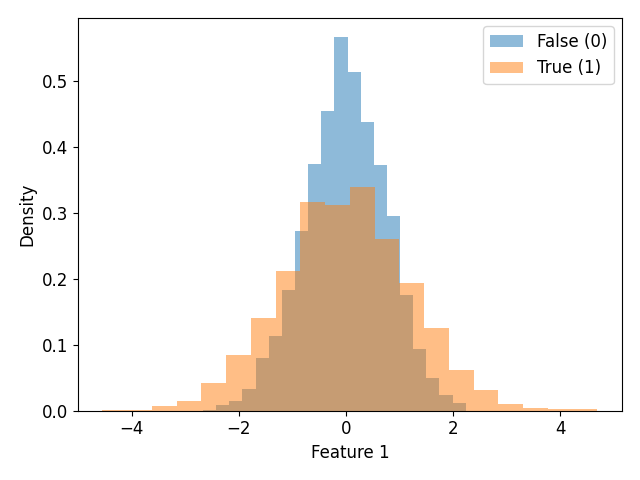
\includegraphics[width=0.62\textwidth]{lab02_hist_1.png}
\caption{Feature 1 --- normalized histogram of the two classes.}
\end{figure}

\paragraph{Q2 --- Features 3 and 4.}
Here the situation is reversed: $|\Delta\mu| \approx 1.35$ for both
features 3 and 4, while the variances are virtually identical between
the two classes ($\approx 0.54$). The two classes separate well by
mean shift. The histograms show two shifted, uni-modal Gaussians.
These are the most informative features in a ``linear-mean-based''
sense.

\begin{figure}[H]
\centering
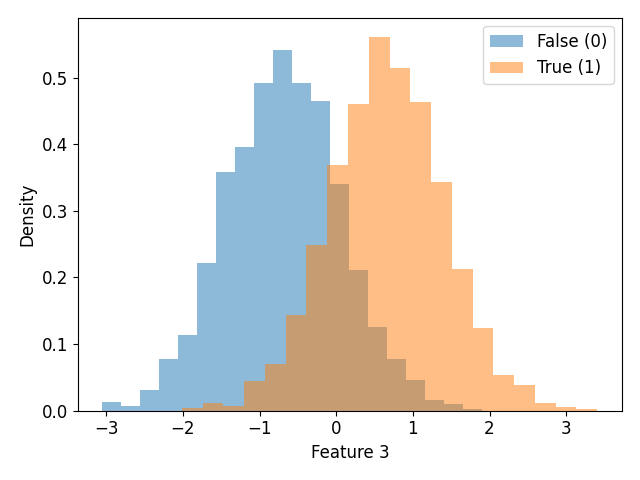
\includegraphics[width=0.62\textwidth]{lab02_hist_3.png}
\caption{Feature 3 --- the two classes separate by mean translation.}
\end{figure}

\paragraph{Q3 --- Features 5 and 6.}
The histograms show a radically different behavior: the genuine class
is clearly \textbf{bi-modal} (two symmetric peaks around $\pm 1$),
while the fake class remains uni-modal and concentrated around 0. The
5--6 scatter plot shows that the genuine class forms \textbf{4
clusters} arranged in a ``square'' around the origin, while the fake
class concentrates in a single central cluster with tails filling the
space. These are non-Gaussian features with a sub-categorical
structure $\rightarrow$ very strong motivation for a GMM with 4+
components on class 1.

\begin{figure}[H]
\centering
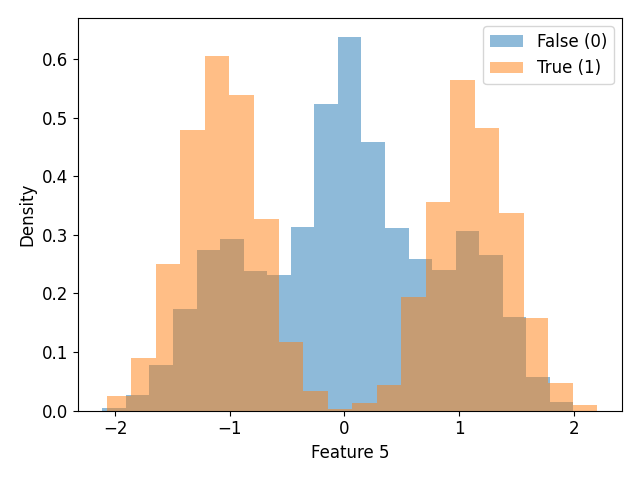
\includegraphics[width=0.55\textwidth]{lab02_hist_5.png}\hspace{0.5em}
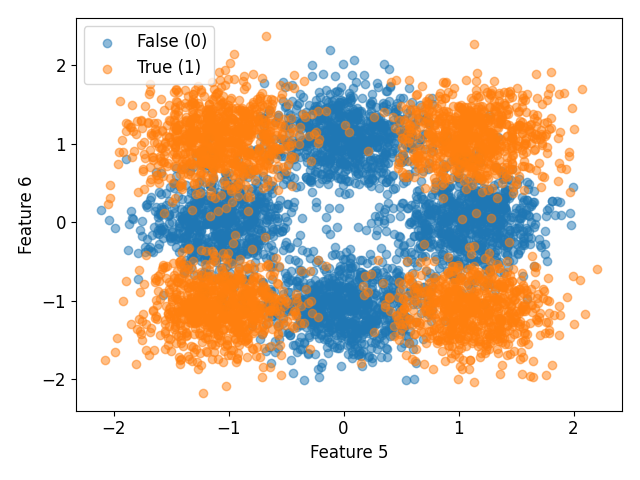
\includegraphics[width=0.40\textwidth]{lab02_scatter_5_6.png}
\caption{(Left) Feature 5: bimodal distribution for the genuine class.
         (Right) Scatter plot of features 5--6: the genuine class
         forms 4 well-separated clusters; the fake class only one
         central cluster.}
\end{figure}

\subsection{Implications for the subsequent models}

\begin{itemize}
\item Features 1--2 $\rightarrow$ a classifier based on means only
      (Tied MVG, LDA, linear LR) \textbf{cannot} discriminate them.
      Models sensitive to different per-class covariances are required
      (full MVG, QDA, kernel SVM, GMM).
\item Features 3--4 $\rightarrow$ discriminable even with ``very poor''
      models such as Tied/LDA.
\item Features 5--6 $\rightarrow$ the multi-cluster structure
      justifies a priori why a GMM with many components will win.
\end{itemize}

%-----------------------------------------------------------------------------
\section{Lab 3 -- Dimensionality reduction (PCA and LDA)}\label{sec:lab3}
%-----------------------------------------------------------------------------

\subsection{Method}

Script \texttt{experiments/lab03\_dimensionality\_reduction.py}, using:
\begin{itemize}
\item \texttt{models/pca.py} --- \texttt{compute\_pca(D, m)} computes
      the eigenvectors of the data covariance matrix via SVD.
\item \texttt{models/lda.py} --- computes $S_B$ (between-class) and
      $S_W$ (within-class) and solves
      \texttt{scipy.linalg.eigh(S\_B, S\_W)} (generalized problem).
\end{itemize}

\textbf{LDA classification pipeline (binary):}
\begin{enumerate}
\item Estimate $U_{\textrm{lda}}$ on $(\mathit{DTR}, \mathit{LTR})$.
\item Project $\mathit{DTR} \rightarrow \mathit{DTR}_{\textrm{lda}}$,
      $\mathit{DVAL} \rightarrow \mathit{DVAL}_{\textrm{lda}}$.
\item \textbf{Fix orientation} so that
      $\mu_{\textrm{lda}}[\textrm{class }0] > \mu_{\textrm{lda}}[\textrm{class }1]$
      (by convention our LLR is $\log p(x|1) - \log p(x|0)$).
\item Threshold ``mean of means'':
      $t = (\mu_{\textrm{lda},0} + \mu_{\textrm{lda},1})/2$.
\item Predict 0 if projection $\geq t$, 1 otherwise.
\end{enumerate}

\subsection{PCA results}

\begin{table}[H]
\centering
\small
\begin{tabular}{lrrrrr}
\toprule
PCA direction   & $\mu$ cls 0 & $\sigma$ cls 0 & $\mu$ cls 1 & $\sigma$ cls 1 & $|\Delta\mu|$ \\
\midrule
1 (principal)   & $-0.955$ & $0.731$ & $+0.940$ & $0.739$ & $\mathbf{1.895}$ \\
2               & $-0.029$ & $0.802$ & $+0.018$ & $1.176$ & $0.046$ \\
3               & $+0.034$ & $1.029$ & $-0.021$ & $0.973$ & $0.055$ \\
4               & $+0.034$ & $0.992$ & $-0.045$ & $1.001$ & $0.079$ \\
5               & $+0.011$ & $0.830$ & $+0.005$ & $1.129$ & $0.005$ \\
6               & $-0.000$ & $0.745$ & $+0.007$ & $0.750$ & $0.007$ \\
\bottomrule
\end{tabular}
\end{table}

Only the first PCA direction has discriminative power
($|\Delta\mu| \approx 1.9$), because it concentrates the information
from features 3--4 (the only ones with markedly different means
between classes). The other directions have practically coincident
means --- the between-class difference is almost entirely in the
covariance, which PCA does not see.

\textbf{Key observation (asked by the PDF):} PCA with $m=6$ is just a
rotation: the clusters (e.g.\ those on features 5--6) remain the same,
just in different coordinates. The post-PCA histograms and scatters
``look'' different but the distances between points are invariant.

\subsection{LDA results}

LDA 1-D (maximum number of directions for a binary problem):

\begin{table}[H]
\centering
\small
\begin{tabular}{lrrrrr}
\toprule
                & $\mu$ cls 0 & $\sigma$ cls 0 & $\mu$ cls 1 & $\sigma$ cls 1 & $|\Delta\mu|$ \\
\midrule
LDA direction 1 & $+1.308$ & $0.996$ & $-1.287$ & $1.004$ & $\mathbf{2.595}$ \\
\bottomrule
\end{tabular}
\end{table}

$|\Delta\mu|=2.6$ is significantly larger than the first PCA direction
(1.9): LDA ``pushes'' the classes further apart by exploiting
$S_B/S_W$ rather than only the total variance.

\begin{figure}[H]
\centering
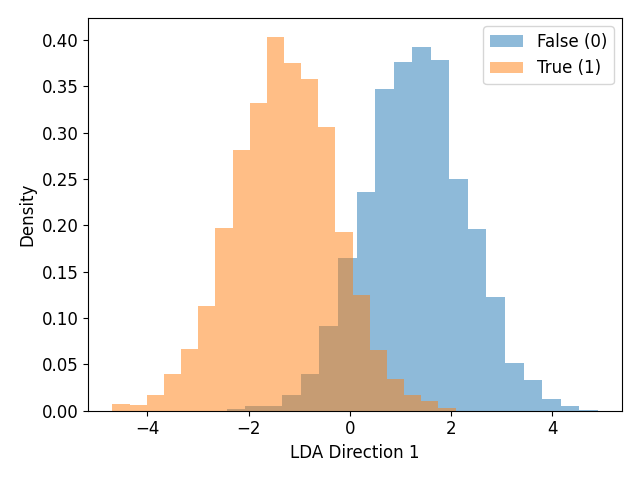
\includegraphics[width=0.62\textwidth]{lab03_hist_lda_1.png}
\caption{1-D LDA projection histogram: classes separate with an
         overlap region around zero.}
\end{figure}

\subsection{LDA-based classification}

\begin{table}[H]
\centering
\begin{tabular}{lrr}
\toprule
Configuration                  & Errors    & Error rate \\
\midrule
``Mean of means'' threshold    & 186 / 2000 & \textbf{9.30 \%} \\
Optimal threshold on DVAL (sweep) & 182 / 2000 & 9.10 \% \\
improvement                    & 4         & 0.20 \% \\
\bottomrule
\end{tabular}
\end{table}

PCA pre-processing + LDA ($m$ = number of PCA components kept):

\begin{table}[H]
\centering
\begin{tabular}{rrr}
\toprule
$m$ & Errors & Error rate \\
\midrule
1   & 187 & 9.35 \% \\
2   & 185 & 9.25 \% \\
3   & 185 & 9.25 \% \\
4   & 185 & 9.25 \% \\
5   & 186 & 9.30 \% \\
6 (no PCA) & 186 & 9.30 \% \\
\bottomrule
\end{tabular}
\end{table}

\subsection{Answers to the Lab 3 project questions}

\begin{itemize}
\item \textbf{PCA effects}: only the first direction discriminates;
      the other 5 carry ``scale'' information that PCA, being
      unsupervised, cannot use. No new clusters become visible because
      PCA is a rotation of the reference frame. There is no ``more
      separation''.
\item \textbf{Is LDA finding a good direction?} Yes: with
      mean-of-means threshold we get 9.30 \% error rate --- the
      recurring reference figure used as a sanity-check value for all
      subsequent labs.
\item \textbf{Does changing the threshold help?} Marginally: only
      from 9.30 \% to 9.10 \% (4 fewer errors). The best threshold
      found ($-0.107$) is not far from the default ($-0.019$).
\item \textbf{Is PCA pre-processing + LDA beneficial?} No, not
      significantly: results stay in $[9.25\%, 9.35\%]$. PCA does not
      help because: (a) the problem is not high-dimensional ($M=6$ is
      already small); (b) LDA is already supervised and gains nothing
      from an unsupervised pre-rotation.
\end{itemize}

%-----------------------------------------------------------------------------
\section{Lab 4 -- Density estimation (1-D Gaussian fit)}\label{sec:lab4}
%-----------------------------------------------------------------------------

\subsection{Method}

Script \texttt{experiments/lab04\_density\_estimation.py}.

For each of the 6 features and each of the 2 classes:
\begin{enumerate}
\item ML estimate: $\mu_{ML} = \frac{1}{N}\sum x_i$,
      $\sigma^2_{ML} = \frac{1}{N}\sum (x_i - \mu_{ML})^2$.
\item Plot the normalized histogram and overlay the fitted Gaussian.
\end{enumerate}

The script outputs a table of the estimates and 6 plots
(\texttt{feature\_1.png} \ldots\ \texttt{feature\_6.png}).

\subsection{Per-class, per-feature ML estimates}

\begin{table}[H]
\centering
\small
\begin{tabular}{rrrr}
\toprule
Feature & Class & $\mu_{ML}$ & $\sigma^2_{ML}$ \\
\midrule
1 & 0 & $+0.0029$ & $0.5696$ \\
1 & 1 & $+0.0005$ & $1.4302$ \\
2 & 0 & $+0.0187$ & $1.4209$ \\
2 & 1 & $-0.0085$ & $0.5783$ \\
3 & 0 & $-0.6809$ & $0.5500$ \\
3 & 1 & $+0.6652$ & $0.5489$ \\
4 & 0 & $+0.6708$ & $0.5360$ \\
4 & 1 & $-0.6642$ & $0.5533$ \\
5 & 0 & $+0.0280$ & $0.6801$ \\
5 & 1 & $-0.0417$ & $1.3178$ \\
6 & 0 & $-0.0058$ & $0.7050$ \\
6 & 1 & $+0.0239$ & $1.2870$ \\
\bottomrule
\end{tabular}
\end{table}

\subsection{Answers to the Lab 4 project questions}

\paragraph{For which features is the Gaussian fit good?}
Features \textbf{1--2--3--4} are reasonably Gaussian: histograms show
a single, approximately symmetric mode, and the Gaussian curve follows
the shape well.

\begin{figure}[H]
\centering
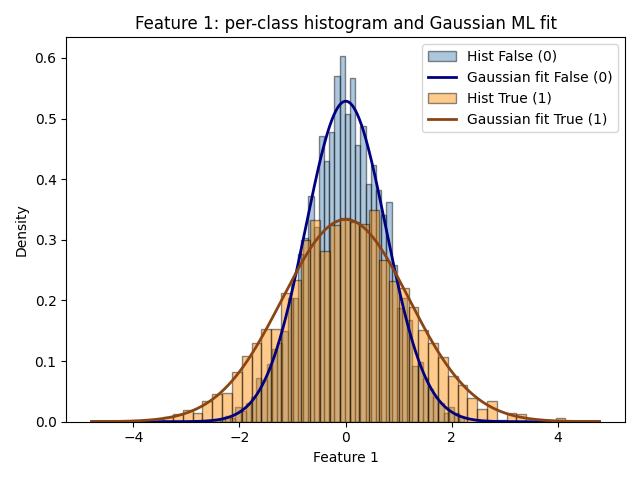
\includegraphics[width=0.48\textwidth]{lab04_feature_1.png}\hfill
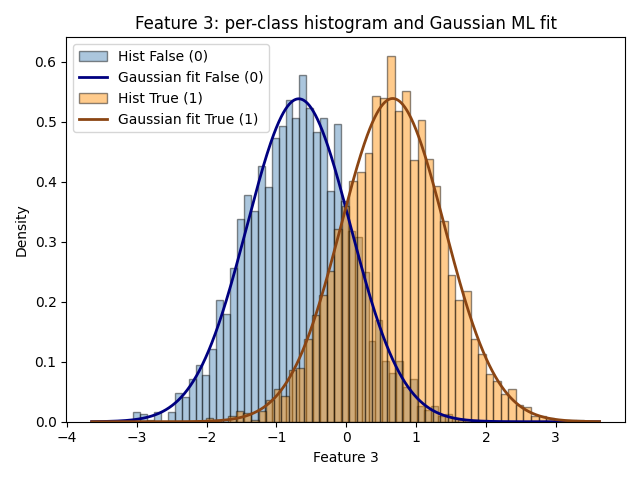
\includegraphics[width=0.48\textwidth]{lab04_feature_3.png}
\caption{Gaussian ML fit for feature 1 (left) and feature 3 (right):
         both are reasonably uni-modal.}
\end{figure}

\paragraph{For which features is the fit poor?}
Features \textbf{5--6}: the genuine-class (label 1) histogram is
clearly \textbf{bimodal}, with two symmetric peaks around $\pm 1$, and
a Gaussian centered at zero with large variance is a very poor
approximation. The fitted Gaussian ``smears'' across both peaks
without capturing them.

\begin{figure}[H]
\centering
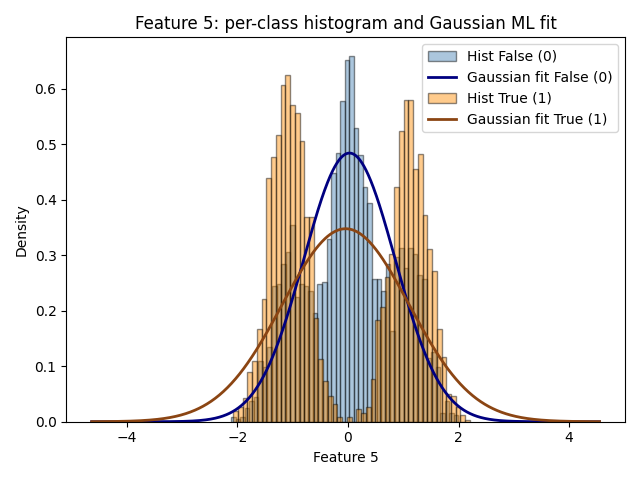
\includegraphics[width=0.62\textwidth]{lab04_feature_5.png}
\caption{Gaussian ML fit for feature 5: the genuine class (orange) is
         bimodal, the fitted Gaussian does not capture it.}
\end{figure}

\paragraph{Consequence for Gaussian models.}
We expect single-Gaussian models (MVG, Naive Bayes, Tied) to
underperform compared to a GMM, especially when features 5--6 are
included. This is confirmed in \S\ref{sec:lab5}: MVG on features
1--4 gets 7.95 \% error rate, MVG on all 6 features 7.00 \% --- the
gain is marginal because a full-covariance MVG struggles with
multimodal features, but the inter-feature covariance helps. The
real quality jump comes with GMM (\S\ref{sec:lab9}).

%-----------------------------------------------------------------------------
\section{Lab 5 -- Generative Gaussian classifiers}\label{sec:lab5}
%-----------------------------------------------------------------------------

\subsection{Method}

Script \texttt{experiments/lab05\_gaussian\_classification.py}, using
\texttt{models/gaussian\_models.py}:
\begin{itemize}
\item \textbf{MVG} (\texttt{Gau\_MVG\_ML\_estimates}): one
      $(\mu_c, \Sigma_c)$ per class.
\item \textbf{Naive Bayes} (\texttt{Gau\_Naive\_ML\_estimates}): as
      MVG but $\Sigma_c \leftarrow \Sigma_c \odot I$ (diagonal only).
\item \textbf{Tied} (\texttt{Gau\_Tied\_ML\_estimates}): $\mu_c$ per
      class but shared $\Sigma$
      $= \frac{1}{N}\sum_c N_c \Sigma_c^*$.
\end{itemize}

\textbf{Inference} (\texttt{compute\_llr}):
\[
   \llr(x) = \log \mathcal{N}(x|\mu_1, \Sigma_1) - \log \mathcal{N}(x|\mu_0, \Sigma_0)
\]
using \texttt{logpdf\_GAU\_ND} for numerical stability. Prediction: 1
if $\llr \geq 0$, 0 otherwise (uniform priors).

\subsection{Covariances and Pearson correlations}

The \textbf{full covariances} of the two classes (summary of the
output), main diagonals:

\begin{itemize}
\item Class 0 (fake):    $[0.60,\ 1.45,\ 0.57,\ 0.54,\ 0.70,\ 0.69]$.
\item Class 1 (genuine): $[1.45,\ 0.55,\ 0.56,\ 0.57,\ 1.34,\ 1.30]$.
\end{itemize}

Off-diagonal terms are all of order $10^{-2}$ or smaller, \textbf{orders
of magnitude smaller} than the diagonal variances.

\textbf{Pearson correlation} (maximum off-diagonal value):
\begin{itemize}
\item Class 0: $\leq 0.034$ (essentially zero).
\item Class 1: maximum $0.049$ between features 3--4.
\end{itemize}

\textbf{Consequence:} features are essentially \textbf{uncorrelated}
within each class. This is why Naive Bayes (which assumes diagonal
covariance) has performance equal or close to MVG: the assumption is
largely true on the data.

\subsection{Classification results (error rate on DVAL)}

\begin{table}[H]
\centering
\begin{tabular}{lr}
\toprule
\multicolumn{2}{c}{\textbf{All 6 features}} \\
\midrule
MVG          & \textbf{7.00 \%} \\
Naive Bayes  & 7.20 \% \\
Tied         & 9.30 \% \\
\bottomrule
\end{tabular}
\hspace{1em}
\begin{tabular}{lr}
\toprule
\multicolumn{2}{c}{\textbf{Features 1--4 only}} \\
\midrule
MVG          & 7.95 \% \\
Naive Bayes  & 7.65 \% \\
Tied         & 9.50 \% \\
\bottomrule
\end{tabular}
\end{table}

\begin{table}[H]
\centering
\begin{tabular}{lr}
\toprule
\multicolumn{2}{c}{\textbf{Features 1--2 only}} \\
\multicolumn{2}{c}{(similar means, different variances)} \\
\midrule
MVG          & 36.50 \% \\
Naive Bayes  & 36.30 \% \\
Tied         & \textbf{49.45 \%} \\
\bottomrule
\end{tabular}
\hspace{1em}
\begin{tabular}{lr}
\toprule
\multicolumn{2}{c}{\textbf{Features 3--4 only}} \\
\multicolumn{2}{c}{(different means, similar variances)} \\
\midrule
MVG          & 9.45 \% \\
Naive Bayes  & 9.45 \% \\
Tied         & 9.40 \% \\
\bottomrule
\end{tabular}
\end{table}

\textbf{PCA + classifiers (on the 6 original features):}

\begin{table}[H]
\centering
\begin{tabular}{rrrr}
\toprule
$m$ & MVG    & Naive Bayes & Tied    \\
\midrule
1   & 9.25 \% & 9.25 \% & 9.35 \% \\
2   & 8.80 \% & 8.85 \% & 9.25 \% \\
3   & 8.80 \% & 9.00 \% & 9.25 \% \\
4   & 8.05 \% & 8.85 \% & 9.25 \% \\
5   & 7.10 \% & 8.75 \% & 9.30 \% \\
6   & 7.00 \% & 8.90 \% & 9.30 \% \\
\bottomrule
\end{tabular}
\end{table}

\subsection{Answers to the Lab 5 project questions}

\begin{itemize}
\item \textbf{Which model is best?} The \textbf{full MVG} on the 6
      features (7.00 \%). Tied is clearly worse (9.30 \%) because it
      imposes a shared covariance across classes, but we know from
      Lab 2 that the variances of features 1, 2, 5, 6 are
      \textbf{very different} between classes: Tied loses this
      information.

\item \textbf{Naive Bayes vs MVG:} essentially on par (7.20 \% vs
      7.00 \%) because features are nearly uncorrelated (Pearson
      $< 0.05$). The diagonality assumption is nearly true.

\item \textbf{Goodness of the Gaussian assumption:} from Lab 4 we
      know features 5--6 are bimodal $\rightarrow$ the assumption is
      violated. Yet dropping 5--6 makes results worse (MVG goes from
      7.00 \% to 7.95 \%). This means that even if a single Gaussian
      does not perfectly model those features, the ``scale''
      information (different variance per class) is still useful.

\item \textbf{Features 1--2 (different variances):} MVG and Naive work
      ($\approx 36 \%$, still high because separation is variance-only);
      Tied collapses to 49 \% (random for a binary problem): with
      nearly equal means and a tied covariance, the two classes become
      indistinguishable.

\item \textbf{Features 3--4 (different means):} all three models get
      $\approx 9.4 \%$, because using the means is enough and variances
      are similar --- Tied is not penalized.

\item \textbf{PCA + Gaussian:} PCA does not improve MVG (7.00 \% at
      $m=6$, 7.10 \% at $m=5$). No benefit. Naive Bayes worsens
      slightly with PCA (PCA reintroduces correlation in the new
      features, violating the naive assumption). Tied is unaffected.
\end{itemize}

\textbf{Sanity check:} \checkmark\ MVG 7.00 \%, Naive 7.20 \%,
Tied 9.30 \%; subset 1--4: 7.95 / 7.65 / 9.50 \%. All expected values
are met.

%-----------------------------------------------------------------------------
\section{Lab 6 -- Bayesian decisions and model evaluation}\label{sec:lab6}
%-----------------------------------------------------------------------------

\subsection{Theoretical framework}

\textbf{Cost matrix} for a binary task:
\[
\mathbf{C} =
\begin{pmatrix}
0       & C_{fn} \\
C_{fp}  & 0
\end{pmatrix}
\]

\textbf{Optimal decision threshold:}
\[
   t = -\log\!\frac{\pi_1 C_{fn}}{(1-\pi_1) C_{fp}}
\]
Predict ``class 1'' if $\llr > t$.

\textbf{Effective prior:}
\[
   \tilde{\pi} = \frac{\pi_1 C_{fn}}{\pi_1 C_{fn} + (1-\pi_1) C_{fp}}
\]
An application $(\pi_1, C_{fn}, C_{fp})$ is, in terms of threshold,
equivalent to $(\tilde{\pi}, 1, 1)$.

\textbf{Normalized DCF:}
\[
   \DCF = \frac{\pi_1 C_{fn} P_{fn} + (1-\pi_1) C_{fp} P_{fp}}{\min(\pi_1 C_{fn},\,(1-\pi_1) C_{fp})}
\]

\begin{itemize}
\item \textbf{actDCF}: DCF using the theoretical threshold $t$.
\item \textbf{minDCF}: minimum DCF over all possible thresholds
      (lower bound; measures pure ``separability'' independent of
      calibration).
\item \textbf{Calibration loss} $= \actDCF - \minDCF$.
\end{itemize}

Implementation in \texttt{utils/evaluation.py}:
\begin{itemize}
\item \texttt{compute\_optimal\_Bayes\_binary\_llr(llr, prior, Cfn, Cfp)}
      computes the theoretical threshold and decisions.
\item \texttt{compute\_minDCF\_binary\_fast} sorts the scores and
      computes all possible $P_{fn}/P_{fp}$ in $O(N\log N)$.
\item \texttt{compute\_actDCF\_binary\_fast} $=$
      \texttt{compute\_empirical\_Bayes\_risk\_binary\_llr\_optimal\_decisions}.
\end{itemize}

\subsection{Applications considered}

The Lab 6 PDF asks to evaluate 5 applications and convert them to
effective priors:

\begin{table}[H]
\centering
\begin{tabular}{lr}
\toprule
$(\pi_1, C_{fn}, C_{fp})$ & $\tilde{\pi}$ \\
\midrule
$(0.5, 1, 1)$                          & 0.5 \\
$(0.9, 1, 1)$                          & 0.9 \\
$(0.1, 1, 1)$                          & 0.1 \\
$(0.5, 1, 9)$ --- strong security      & 0.1 \\
$(0.5, 9, 1)$ --- ease of use          & 0.9 \\
\bottomrule
\end{tabular}
\end{table}

\textbf{Interpretation:} increasing $C_{fp}$ (penalty for false
positives $=$ accepting a fake) lowers the effective prior of genuine.
``Strong security'' ($\tilde{\pi}=0.1$) is equivalent, decision-wise,
to the ``many impostors'' application ($\pi_1=0.1$). The three
canonical effective priors we examine from now on are
\textbf{0.1, 0.5, 0.9}.

\subsection{DCF results for the three Gaussian models}

\begin{table}[H]
\centering
\begin{tabular}{lrrrr}
\toprule
Model         & $\tilde{\pi}$ & actDCF & minDCF & cal-loss \\
\midrule
MVG           & 0.1 & 0.3051 & 0.2629 & 0.0422 \\
Naive Bayes   & 0.1 & 0.3022 & 0.2570 & 0.0452 \\
Tied          & 0.1 & 0.4061 & 0.3628 & 0.0432 \\
\midrule
\textbf{MVG}  & \textbf{0.5} & \textbf{0.1399} & \textbf{0.1302} & \textbf{0.0098} \\
Naive Bayes   & 0.5 & 0.1439 & 0.1311 & 0.0128 \\
Tied          & 0.5 & 0.1860 & 0.1812 & 0.0048 \\
\midrule
MVG           & 0.9 & 0.4001 & 0.3423 & 0.0577 \\
Naive Bayes   & 0.9 & 0.3893 & 0.3510 & 0.0383 \\
Tied          & 0.9 & 0.4626 & 0.4421 & 0.0204 \\
\bottomrule
\end{tabular}
\end{table}

\subsection{Bayes Error Plot}

Plot with prior log-odds $\in [-4, +4]$, one column for each of the 3
models:

\begin{figure}[H]
\centering
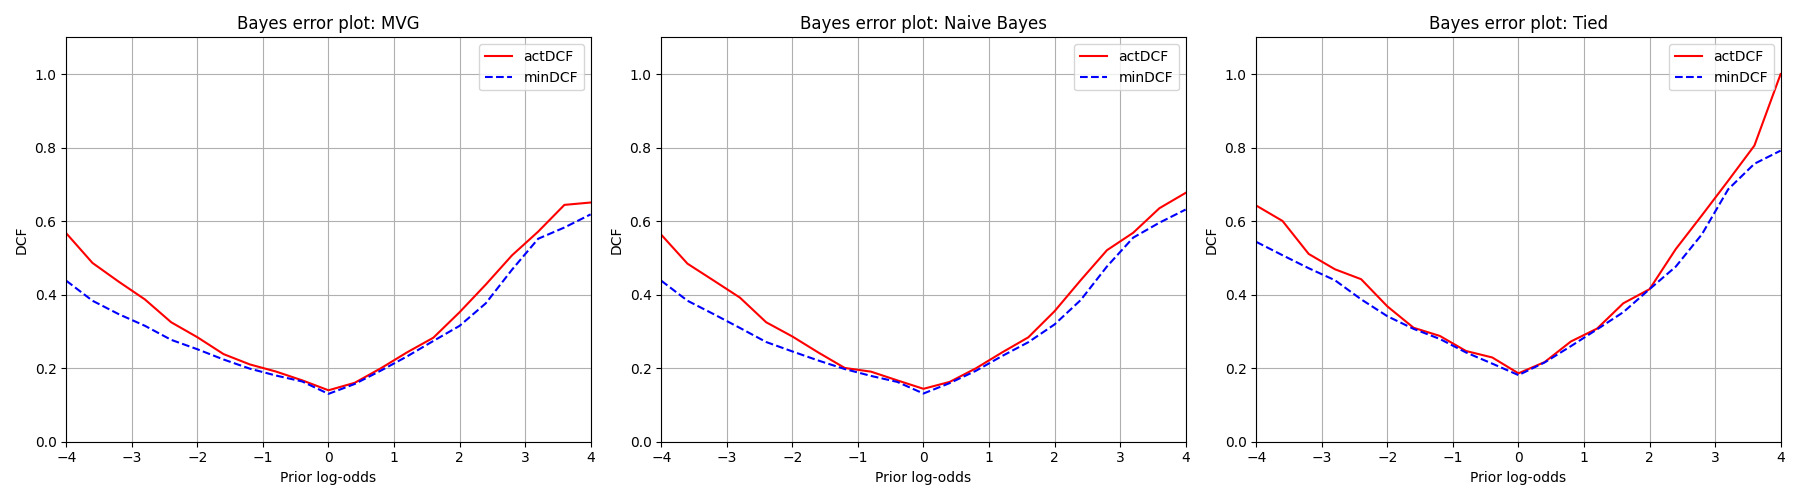
\includegraphics[width=\textwidth]{lab06_bayes_error_plots.png}
\caption{Bayes error plot for the 3 Gaussian classifiers. The actDCF
         curve (red) lies on top of the minDCF (dashed blue) and
         separates in the ``tails''.}
\end{figure}

\subsection{Answers to the Lab 6 project questions}

\begin{itemize}
\item \textbf{Which model is best in minDCF?}
      For $\tilde{\pi}=0.5$: MVG (0.130). For $\tilde{\pi}=0.1$ and
      $0.9$: Naive Bayes (0.257 and 0.351). Tied is always the worst.

\item \textbf{Ranking consistent across applications?} Almost: Tied is
      always last. MVG and Naive swap slightly: MVG wins at
      $\tilde{\pi}=0.5$, Naive at $0.1$ and $0.9$ --- consistent with
      the fact that features are nearly uncorrelated (Naive loses
      little) and Naive has fewer parameters $\rightarrow$ less
      variance $\rightarrow$ better in the application ``tails''.

\item \textbf{Are the models well calibrated?} For $\tilde{\pi}=0.5$
      yes (calibration loss $<1\%$ of minDCF in absolute value). For
      the extreme applications $\tilde{\pi}=0.1$ and $0.9$ there is a
      $\sim 5\%$ gap: the models are \textbf{suboptimally calibrated}
      for ``asymmetric'' applications.

\item \textbf{Bayes error plot:} the actDCF curve separates from the
      minDCF in the tails log-odds $=\pm 4$. For Tied, actDCF blows up
      faster on the high $\tilde{\pi}$ side (log-odds $>2$): a sign of
      strong miscalibration for high-class-1-prior applications.
\end{itemize}

\textbf{Sanity check:} \checkmark\ MVG @ $\tilde{\pi}=0.5$:
actDCF $\approx 0.140$, minDCF $\approx 0.130$.

%-----------------------------------------------------------------------------
\section{Lab 7 -- Logistic Regression}\label{sec:lab7}
%-----------------------------------------------------------------------------

\subsection{Theoretical framework}

\textbf{Standard (non-weighted) model} (loss $=$ average cross-entropy
$+$ regularization):
\[
J(w, b) = \frac{\lambda}{2}\|w\|^2
       + \frac{1}{n}\sum_{i=1}^{n} \log\!\left(1 + e^{-z_i(w^Tx_i + b)}\right),
\quad z_i = 2c_i - 1
\]

\textbf{Prior-weighted model} (to simulate a prior $\pi_T$):
\[
J(w, b) = \frac{\lambda}{2}\|w\|^2
       + \sum_i \xi_i \log\!\left(1 + e^{-z_i(w^Tx_i + b)}\right),\quad
\xi_i =
\begin{cases}
\pi_T / n_T       & z_i = +1 \\
(1-\pi_T) / n_F   & z_i = -1
\end{cases}
\]

\textbf{Gradients} (closed form, to speed up L-BFGS):
\[
G_i = \frac{-z_i}{1 + e^{z_i(w^Tx_i + b)}};\quad
\nabla_w J = \lambda w + \frac{1}{n}\sum_i G_i x_i;\quad
\partial_b J = \frac{1}{n}\sum_i G_i
\]

\textbf{Scoring} $\rightarrow$ \textbf{LLR-like:} the LR model gives a
score $s(x) = w^T x + b$ that behaves as a log-posterior ratio based
on the empirical training-set prior. To make it compatible with our
theoretical threshold $t = -\log(\pi_T/(1-\pi_T))$ we have to
\textbf{subtract the log-odds of the training prior}:
\begin{itemize}
\item Standard LR:
      $s_{\textrm{llr}} = s - \log(\pi_{\textrm{emp}} / (1-\pi_{\textrm{emp}}))$.
\item Prior-weighted LR (target $\pi_T$):
      $s_{\textrm{llr}} = s - \log(\pi_T / (1-\pi_T))$.
\end{itemize}

\textbf{Quadratic LR:} expansion
$\phi(x) = [\textrm{vec}(xx^T),\,x]$ (42-D from 6 features).
Implemented in \texttt{expand\_features\_quadratic}.

\subsection{Experiment setup}

$\lambda \in$ \texttt{numpy.logspace(-4, 2, 13)} (13 values from
$10^{-4}$ to $10^{2}$). Target application: $\pi_T = 0.1$.

\subsection{Standard LR on the full training set (4000 samples)}

\begin{table}[H]
\centering
\small
\begin{tabular}{rrrr}
\toprule
$\lambda$  & $J^*(w,b)$    & actDCF & minDCF \\
\midrule
$10^{-4}$  & $2.378\cdot 10^{-1}$ & 0.4021 & 0.3640 \\
$3.2\cdot 10^{-4}$ & $2.391\cdot 10^{-1}$ & 0.4051 & 0.3650 \\
$10^{-3}$  & $2.431\cdot 10^{-1}$ & 0.4130 & 0.3650 \\
$3.2\cdot 10^{-3}$ & $2.543\cdot 10^{-1}$ & 0.4297 & 0.3641 \\
$\mathbf{10^{-2}}$ & $2.816\cdot 10^{-1}$ & 0.4568 & $\mathbf{0.3611}$ \\
$3.2\cdot 10^{-2}$ & $3.353\cdot 10^{-1}$ & 0.5805 & 0.3621 \\
$10^{-1}$ & $4.198\cdot 10^{-1}$ & 0.8522 & 0.3641 \\
$1$       & $6.108\cdot 10^{-1}$ & 1.0000 & 0.3640 \\
$10^{2}$  & $6.920\cdot 10^{-1}$ & 1.0000 & 0.3620 \\
\bottomrule
\end{tabular}
\end{table}

\begin{figure}[H]
\centering
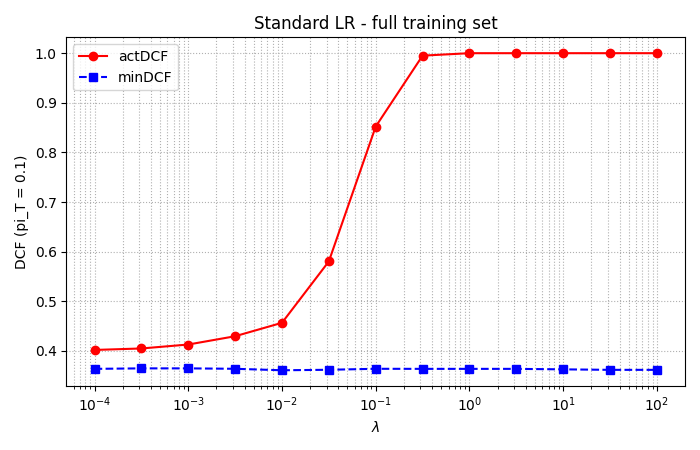
\includegraphics[width=0.70\textwidth]{lab07_01_std_full.png}
\caption{Standard LR on full DTR: minDCF essentially flat, actDCF
         blows up as $\lambda$ grows.}
\end{figure}

\textbf{Observation:} minDCF is essentially flat between $\sim 0.361$
and $\sim 0.365$ --- regularization has no effect on separability
because we have 4000 samples and only 7 parameters (6 + bias). actDCF
instead blows up with $\lambda$: weights are ``shrunk'' and the prior
offset is no longer enough to calibrate them; the score loses its
probabilistic interpretation.

\subsection{Standard LR on the reduced dataset (1 out of 50, 80 samples)}

\begin{table}[H]
\centering
\small
\begin{tabular}{rrrr}
\toprule
$\lambda$  & $J^*(w,b)$    & actDCF & minDCF \\
\midrule
$10^{-4}$ & $1.198\cdot 10^{-1}$ & 0.9780 & 0.4466 \\
$10^{-3}$ & $1.386\cdot 10^{-1}$ & 0.7466 & 0.4487 \\
$10^{-2}$ & $2.070\cdot 10^{-1}$ & 0.4652 & 0.4407 \\
$3.2\cdot 10^{-2}$ & $2.759\cdot 10^{-1}$ & 0.4830 & 0.4147 \\
$10^{-1}$ & $3.738\cdot 10^{-1}$ & 0.7164 & 0.3988 \\
$3.2\cdot 10^{-1}$ & $4.895\cdot 10^{-1}$ & 0.9792 & 0.3888 \\
$\mathbf{10^{+1}}$ & $6.752\cdot 10^{-1}$ & 1.0000 & $\mathbf{0.3783}$ \\
$3.2\cdot 10^{+1}$ & $6.839\cdot 10^{-1}$ & 1.0000 & 0.3793 \\
$10^{+2}$ & $6.868\cdot 10^{-1}$ & 1.0000 & 0.3783 \\
\bottomrule
\end{tabular}
\end{table}

\begin{figure}[H]
\centering
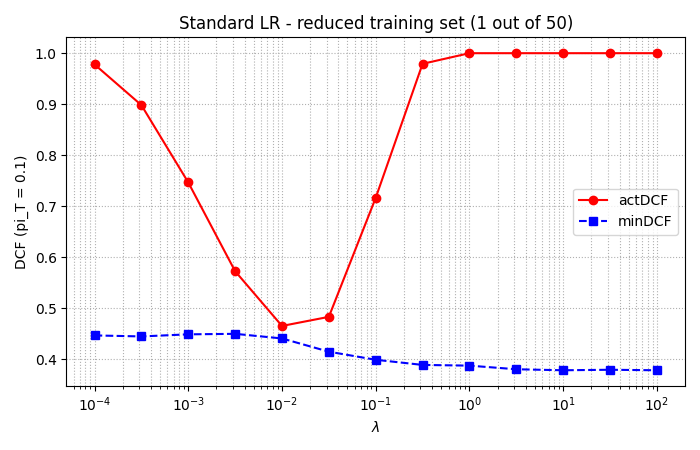
\includegraphics[width=0.70\textwidth]{lab07_02_std_reduced.png}
\caption{Standard LR on reduced DTR (80 samples): regularization is
         critical. Classic ``U'' shape of the bias/variance trade-off.}
\end{figure}

\textbf{Observation:} now regularization \textbf{is critical}. With no
regularization ($\lambda$ small), the 80 samples cause overfitting
$\rightarrow$ minDCF at 0.447. Increasing $\lambda$ reduces overfitting
$\rightarrow$ minDCF drops to 0.378.

\subsection{Prior-weighted LR ($\pi_T=0.1$, full DTR)}

\begin{table}[H]
\centering
\small
\begin{tabular}{rrrr}
\toprule
$\lambda$ & $J^*$ & actDCF & minDCF \\
\midrule
$10^{-4}$ & $1.296\cdot 10^{-1}$ & 0.4071 & 0.3721 \\
$10^{-3}$ & $1.343\cdot 10^{-1}$ & 0.4129 & 0.3699 \\
$10^{-2}$ & $1.643\cdot 10^{-1}$ & 0.4487 & 0.3630 \\
$\mathbf{3.2\cdot 10^{+1}}$ & $3.246\cdot 10^{-1}$ & 1.0000 & $\mathbf{0.3620}$ \\
\bottomrule
\end{tabular}
\end{table}

\begin{figure}[H]
\centering
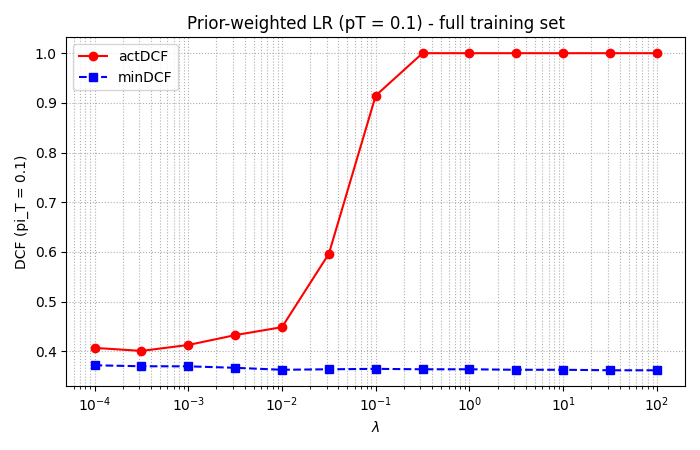
\includegraphics[width=0.70\textwidth]{lab07_03_weighted_full.png}
\caption{Prior-weighted LR on full DTR: results almost identical to
         the non-weighted model (balanced dataset).}
\end{figure}

\textbf{Observation:} for this task there is \textbf{no significant
advantage} in the prior-weighted model: the dataset is balanced
($\pi_{\textrm{emp}} \approx 0.5$), so weight substitutions do not
substantially change the geometry of the problem.

\subsection{Quadratic LR (full DTR)}

\begin{table}[H]
\centering
\small
\begin{tabular}{rrrr}
\toprule
$\lambda$ & $J^*$ & actDCF & minDCF \\
\midrule
$10^{-4}$ & $1.514\cdot 10^{-1}$ & 0.2768 & 0.2602 \\
$3.2\cdot 10^{-4}$ & $1.535\cdot 10^{-1}$ & 0.2656 & 0.2612 \\
$10^{-3}$ & $1.596\cdot 10^{-1}$ & 0.2765 & 0.2587 \\
$3.2\cdot 10^{-3}$ & $1.752\cdot 10^{-1}$ & 0.2771 & 0.2527 \\
$10^{-2}$ & $2.086\cdot 10^{-1}$ & 0.3464 & 0.2487 \\
$\mathbf{3.2\cdot 10^{-2}}$ & $2.686\cdot 10^{-1}$ & 0.4972 & $\mathbf{0.2436}$ \\
$10^{-1}$ & $3.595\cdot 10^{-1}$ & 0.7520 & 0.2466 \\
$3.2\cdot 10^{-1}$ & $4.717\cdot 10^{-1}$ & 0.9623 & 0.2629 \\
\bottomrule
\end{tabular}
\end{table}

\begin{figure}[H]
\centering
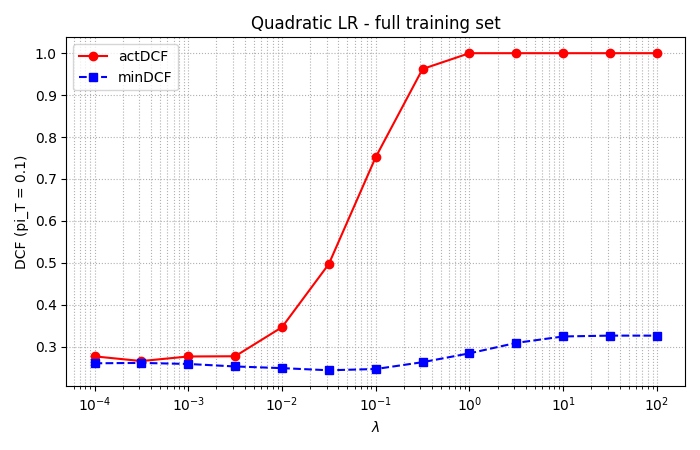
\includegraphics[width=0.70\textwidth]{lab07_04_quadratic_full.png}
\caption{Quadratic LR: sharp qualitative jump compared with linear.
         Regularization is now useful (42 parameters vs 7).}
\end{figure}

\textbf{Observation:} sharp qualitative jump compared with the linear
model. Best minDCF (0.244) is comparable to MVG (0.263). The
quadratic space captures \textbf{feature 5--6 interactions} (the 4
clusters) that the linear model cannot see.

\subsection{Final comparison at target $\pi_T = 0.1$}

\begin{table}[H]
\centering
\begin{tabular}{lrrl}
\toprule
Model                            & actDCF  & minDCF           & hyper \\
\midrule
Gaussian MVG                     & 0.3051  & 0.2629           & --- \\
Gaussian Naive Bayes             & 0.3022  & 0.2570           & --- \\
Gaussian Tied                    & 0.4061  & 0.3628           & --- \\
Standard LR (best $\lambda$)     & 0.4568  & 0.3611           & $\lambda=10^{-2}$ \\
Prior-weighted LR (best $\lambda$)& 1.0000 & 0.3620           & $\lambda=32$ \\
\textbf{Quadratic LR (best $\lambda$)} & 0.4972 & \textbf{0.2436} & $\lambda=3.2\cdot 10^{-2}$ \\
\bottomrule
\end{tabular}
\end{table}

\subsection{Answers to the Lab 7 project questions}

\begin{itemize}
\item \textbf{Effect of $\lambda$ on the full dataset:} negligible on
      minDCF (separability), critical for actDCF (calibration).
      For $\lambda \rightarrow \infty$ the weights collapse to zero
      and the score becomes a constant $\rightarrow$ DCF $= 1$.

\item \textbf{Effect of $\lambda$ on the reduced dataset:} classic
      bias/variance trade-off --- regularization prevents overfitting
      in the few-samples regime.

\item \textbf{Prior-weighted vs standard:} no advantage for this task
      (balanced dataset).

\item \textbf{Quadratic LR:} halves the minDCF of all linear/MVG
      models, confirming that the problem has \textbf{non-linear
      separation}.

\item \textbf{Comparison with Gaussian:}
      \begin{itemize}
      \item Linear LR $\approx$ Tied Gaussian (both linear boundary):
            0.361 vs 0.363.
      \item Quadratic LR $>$ MVG (both quadratic boundary):
            0.244 vs 0.263. The difference is because quadratic LR is
            discriminative while MVG is generative.
      \item Naive Bayes is competitive because features are nearly
            uncorrelated.
      \end{itemize}
\end{itemize}

%-----------------------------------------------------------------------------
\section{Lab 8 -- Support Vector Machines}\label{sec:lab8}
%-----------------------------------------------------------------------------

\subsection{Theoretical framework}

\textbf{Linear primal SVM} (with the extended-feature trick to remove
the $\sum \alpha_i z_i = 0$ constraint):
\[
\hat{J}(\hat{w}) = \frac{1}{2}\|\hat{w}\|^2
                 + C \sum_{i} \max\bigl(0,\,1 - z_i \hat{w}^T \hat{x}_i\bigr),
\quad \hat{x} = [x;\,K]
\]

\textbf{Dual:}
\[
\hat{L}^D(\alpha) = \frac{1}{2}\alpha^T \hat{H}\alpha - \alpha^T \mathbf{1},
\qquad 0 \leq \alpha_i \leq C
\]
with $\hat{H}_{ij} = z_i z_j (x_i^T x_j + K^2)$ in the linear case, or
$\hat{H}_{ij} = z_i z_j (k(x_i, x_j) + \xi)$ with a kernel.

\textbf{Recovering the primal:} $w^* = \sum \alpha_i z_i x_i$,
$b^* = K \cdot \sum \alpha_i z_i$.

\textbf{Test-sample score:}
$s(x) = \sum \alpha_i z_i k(x_i, x) + \xi \sum \alpha_i z_i$.

\textbf{Important:} SVM scores are \textbf{not LLRs}. actDCF is
computed as if they were, but we expect miscalibration (sometimes
drastic). Only minDCF is meaningful as a measure of separability.

\textbf{Kernels} available in \texttt{models/svm.py}:
\begin{itemize}
\item Polynomial: $k(x_1, x_2) = (x_1^T x_2 + c)^d$. For $c=1$ it
      implicitly includes the regularized bias; for $c=0$ it does not.
\item RBF: $k(x_1, x_2) = \exp(-\gamma\|x_1 - x_2\|^2)$. Does not
      include bias $\rightarrow \xi=1$.
\end{itemize}

\subsection{Experiment setup}

\begin{itemize}
\item Linear: $C \in$ \texttt{logspace(-5, 0, 11)}, $K=1$.
      Test on both original and centered data.
\item Poly $d=2$, $c=1$, $\xi=0$, $C \in$ \texttt{logspace(-5, 0, 11)}.
\item RBF: grid $\gamma \in \{e^{-4}, e^{-3}, e^{-2}, e^{-1}\}$,
      $C \in$ \texttt{logspace(-3, 2, 11)}, $\xi=1$.
\item (Optional) Poly $d=4$, $c=1$, $\xi=0$.
\end{itemize}

\subsection{Linear SVM results (summary)}

\paragraph{Non-centered.}
\begin{table}[H]
\centering
\small
\begin{tabular}{rrrrrr}
\toprule
$C$  & primal      & dual         & duality gap & actDCF & minDCF \\
\midrule
$10^{-5}$            & $4.0\cdot 10^{-2}$ & $-0$ & $4\cdot 10^{-2}$ & 1.000 & 1.000 \\
$10^{-4}$            & $3.29\cdot 10^{-1}$ & $3.29\cdot 10^{-1}$ & $2.7\cdot 10^{-9}$ & 1.000 & 0.364 \\
$10^{-2}$            & $1.14\cdot 10^{+1}$ & $1.14\cdot 10^{+1}$ & $2.2\cdot 10^{-4}$ & 0.673 & 0.363 \\
$\mathbf{3.2\cdot 10^{-1}}$ & $3.06\cdot 10^{+2}$ & $3.06\cdot 10^{+2}$ & $1.3\cdot 10^{-2}$ & 0.495 & $\mathbf{0.358}$ \\
$1.0$                & $9.63\cdot 10^{+2}$ & $9.62\cdot 10^{+2}$ & $5.5\cdot 10^{-2}$ & 0.486 & 0.358 \\
\bottomrule
\end{tabular}
\end{table}

\paragraph{Centered (DTR mean subtracted from DTR and DVAL).}
Best: $C=10^{-1}$, primal $\approx 9.86\cdot 10^{+1}$, actDCF $=0.518$,
minDCF $\mathbf{=0.357}$.

\begin{figure}[H]
\centering
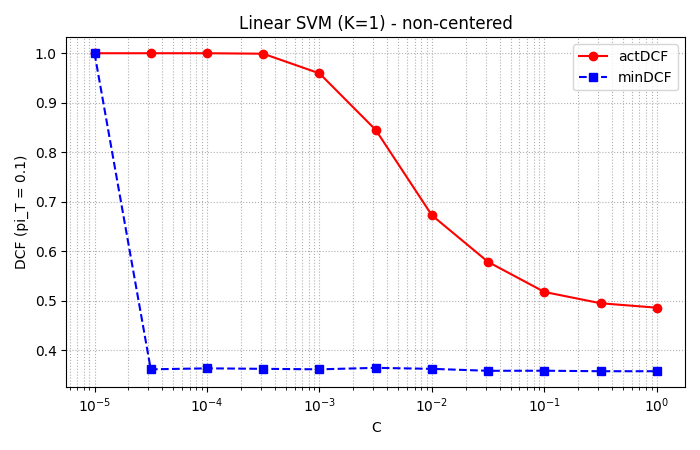
\includegraphics[width=0.70\textwidth]{lab08_01_linear.png}
\caption{Linear SVM (non-centered): minDCF converges to $\sim 0.358$
         for large enough $C$, actDCF stays above 0.5.}
\end{figure}

\textbf{Observation:} best minDCF $\approx 0.358$ (slightly better than
linear LR at 0.361). Centering does not substantially change the
results. actDCF remains very high ($\geq 0.49$ at best): the linear SVM
is heavily miscalibrated for $\pi_T = 0.1$.

\subsection{Polynomial kernel SVM ($d=2$, $c=1$, $\xi=0$)}

\begin{table}[H]
\centering
\small
\begin{tabular}{rrrrr}
\toprule
$C$               & primal              & dual                 & actDCF & minDCF \\
\midrule
$3.2\cdot 10^{-5}$ & $1.08\cdot 10^{-1}$ & $1.08\cdot 10^{-1}$  & 1.000 & 0.246 \\
$10^{-3}$          & $1.28$              & $1.28$               & 0.920 & 0.257 \\
$\mathbf{3.2\cdot 10^{-2}}$ & $2.18\cdot 10^{+1}$ & $2.18\cdot 10^{+1}$ & 0.466 & $\mathbf{0.246}$ \\
$10^{-1}$          & $6.37\cdot 10^{+1}$ & $6.37\cdot 10^{+1}$  & 0.408 & 0.249 \\
$1.0$              & $6.03\cdot 10^{+2}$ & $6.02\cdot 10^{+2}$  & 0.389 & 0.258 \\
\bottomrule
\end{tabular}
\end{table}

\begin{figure}[H]
\centering
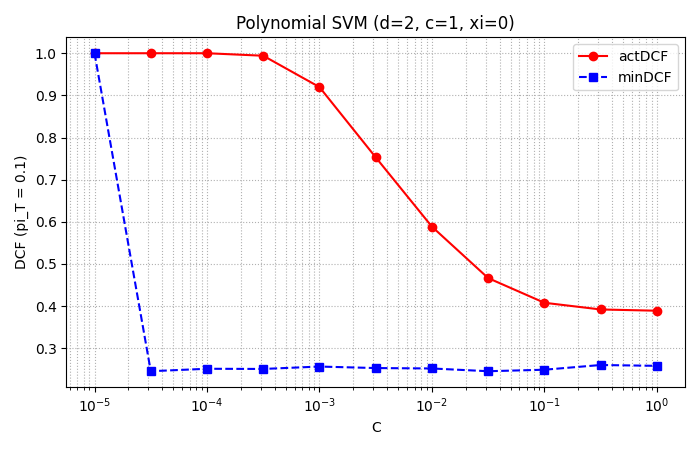
\includegraphics[width=0.70\textwidth]{lab08_03_poly_d2.png}
\caption{Polynomial SVM $d=2$: best minDCF $\approx 0.246$, comparable
         to Quadratic LR.}
\end{figure}

\textbf{Observation:} the poly $d=2$ kernel essentially implements the
same expanded feature space as the Quadratic LR.

\subsection{RBF kernel SVM ($\gamma \times C$ grid, $\xi=1$)}

Sweep over 4 $\gamma$ $\times$ 11 $C$ $= 44$ models. Summary table
(best row per $\gamma$):

\begin{table}[H]
\centering
\begin{tabular}{lrrr}
\toprule
$\gamma$                & $C$-best & minDCF-best & actDCF \\
\midrule
$e^{-4} \approx 0.018$  & $10$    & 0.241 & 0.314 \\
$e^{-3} \approx 0.050$  & $3.2$   & 0.239 & 0.467 \\
$\mathbf{e^{-2} \approx 0.135}$ & $\mathbf{32}$ & $\mathbf{0.173}$ & 0.423 \\
$e^{-1} \approx 0.368$  & $1.0$   & 0.183 & 0.901 \\
\bottomrule
\end{tabular}
\end{table}

\begin{figure}[H]
\centering
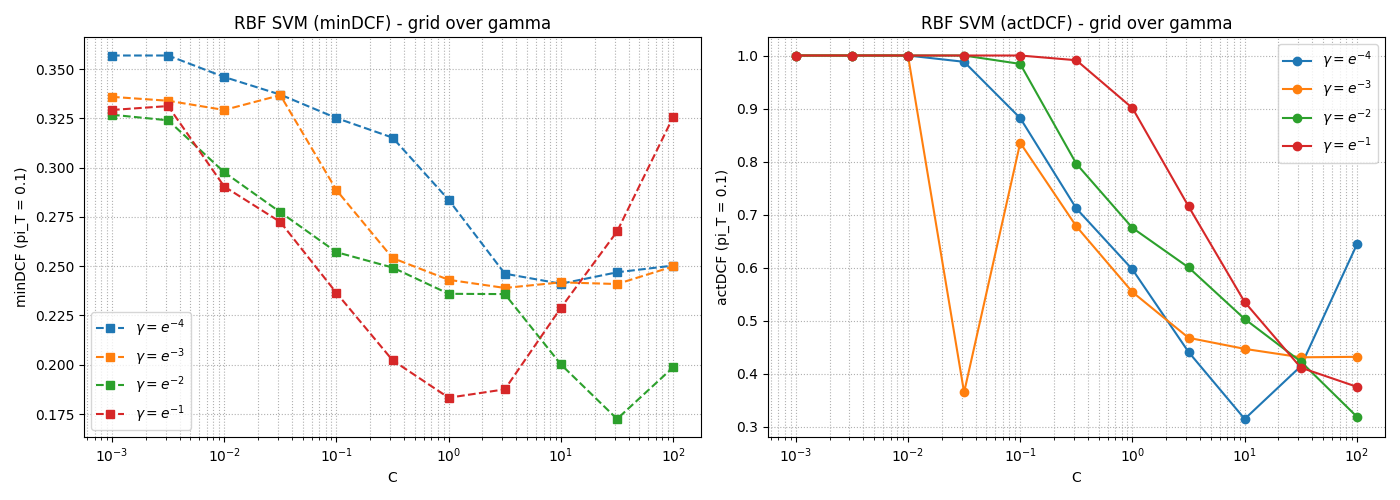
\includegraphics[width=\textwidth]{lab08_04_rbf_grid.png}
\caption{RBF SVM grid: minDCF (left) and actDCF (right) as a function
         of $C$, one line per $\gamma$. Sweet spot at $\gamma=e^{-2}$,
         $C=32$.}
\end{figure}

\textbf{Global best:} $\gamma = e^{-2} \approx 0.135$, $C = 32$,
$\minDCF = \mathbf{0.1725}$, actDCF $= 0.4226$.

\textbf{Observation:} the RBF kernel is the first model in the whole
project to go below $0.20$ minDCF. Its ability to draw non-parametric
decision boundaries captures the ``cluster'' structure of features
5--6 well.

\subsection{(Optional) Poly $d=4$}

\begin{table}[H]
\centering
\begin{tabular}{rrr}
\toprule
$C$               & actDCF & minDCF \\
\midrule
$3.2\cdot 10^{-3}$ & 0.320 & $\mathbf{0.177}$ \\
$10^{-3}$          & 0.399 & 0.178 \\
\bottomrule
\end{tabular}
\end{table}

Poly $d=4$ reaches minDCF $\approx 0.177$, close to the RBF best.
Confirms that the problem is well separated by high-degree polynomial
surfaces, because features 5--6 form a structure well approximated by
high-order cross products.

\subsection{Final comparison ($\pi_T = 0.1$)}

\begin{table}[H]
\centering
\begin{tabular}{lrrl}
\toprule
SVM model                          & actDCF & minDCF & hyper \\
\midrule
Linear (non-centered, best $C$)    & 0.495 & 0.358          & $C=0.32$ \\
Linear (centered, best $C$)        & 0.518 & 0.357          & $C=0.1$ \\
Poly $d=2$ (best $C$)              & 0.466 & 0.246          & $C=3.2\cdot 10^{-2}$ \\
\textbf{RBF (best $\gamma$, $C$)}  & 0.423 & \textbf{0.173} & $\gamma=e^{-2}, C=32$ \\
(opt) Poly $d=4$ (best $C$)        & 0.320 & 0.177          & $C=3.2\cdot 10^{-3}$ \\
\bottomrule
\end{tabular}
\end{table}

\subsection{Answers to the Lab 8 project questions}

\begin{itemize}
\item \textbf{Linear SVM and regularization:} small $C$ (strong
      regularization) $\rightarrow$ model collapses, $\minDCF=1$.
      Large $C$: minDCF stabilizes around $\sim 0.358$. Calibration
      always poor (actDCF $\gg$ minDCF).
\item \textbf{Centered data:} no significant difference. Features were
      already zero-mean.
\item \textbf{Comparison with linear LR and Tied:} essentially
      equivalent in minDCF ($\sim 0.36$).
\item \textbf{Polynomial $d=2$:} halves the minDCF compared with
      linear (0.246 vs 0.358). Consistent with the fact that features
      require quadratic boundaries. Calibration still poor (actDCF
      $\approx 0.47$).
\item \textbf{RBF:} best model in this family. $\gamma$ controls
      kernel ``width'': too large ($e^{-1}$) $\rightarrow$ local
      overfit; too small ($e^{-4}$) $\rightarrow$ almost flat kernel.
      Sweet spot ($\gamma=e^{-2}$) is the best.
\item \textbf{Score calibration:} all SVMs are miscalibrated on this
      application.
\item \textbf{(opt) Poly $d=4$:} similar to RBF. The PDF hint links
      this choice to the geometric structure of the dataset: a
      degree-4 kernel can implement products like $y_5^2 y_6^2$ or
      $y_5 y_6$ that separate the 4 clusters in features 5--6 well.
\end{itemize}

%-----------------------------------------------------------------------------
\section{Lab 9 -- Gaussian Mixture Models}\label{sec:lab9}
%-----------------------------------------------------------------------------

\subsection{Theoretical framework}

\textbf{GMM model:} mixture density of $M$ Gaussians:
\[
f_X(x) = \sum_{g=1}^{M} w_g \, \mathcal{N}(x|\mu_g, \Sigma_g)
\]
with $\sum w_g = 1$.

\textbf{EM algorithm} (in \texttt{models/gmm.py::\_em\_iteration}):
\begin{itemize}
\item \textbf{E-step:} responsibilities
      $\gamma_{g,i} = P(G=g\,|\,x_i)
       = w_g \mathcal{N}(x_i|\mu_g, \Sigma_g)/f_X(x_i)$, computed in
      log-domain via \texttt{logsumexp}.
\item \textbf{M-step:} statistics $Z_g, F_g, S_g$ $\rightarrow$ update
      of $\mu_g, \Sigma_g, w_g$.
\end{itemize}

\textbf{Covariance variants:}
\begin{itemize}
\item Full: no constraint.
\item Diagonal: $\Sigma_g \leftarrow \Sigma_g \odot I$ after M-step.
\item Tied (all components share $\Sigma$ within a GMM):
      $\Sigma \leftarrow \sum w_g \Sigma_g$ after M-step.
\end{itemize}

\textbf{Eigenvalue thresholding}
(\texttt{smooth\_covariance\_matrix}): constraint
$\lambda_{\min}(\Sigma) \geq \psi$ ($\psi=10^{-2}$) to avoid
degenerate solutions.

\textbf{LBG initialization:} starts from 1 Gaussian (ML estimate),
then doubles the number of components by splitting each along the
leading eigenvector direction
($d = U_{[:,0]} \cdot \sqrt{s_0} \cdot \alpha$, with $\alpha=0.1$),
and applies EM to the doubled GMM.

\textbf{LLR for binary classification:}
$\llr(x) = \log \textrm{GMM}_1(x) - \log \textrm{GMM}_0(x)$.

\subsection{Experiment setup}

\begin{itemize}
\item For each class, $K \in \{1, 2, 4, 8, 16\}$. We explore
      \textbf{the full Cartesian product} $5 \times 5 = 25$
      combinations ($K_0$ for fake, $K_1$ for genuine).
\item $\psi = 10^{-2}$, $\alpha_{\textrm{LBG}} = 0.1$,
      EM stopping criterion: $\Delta$ avg-ll $\leq 10^{-6}$.
\item Target: $\pi_T = 0.1$.
\end{itemize}

\subsection{Full-covariance GMM results}

\paragraph{minDCF matrix (row $K_0$, column $K_1$).}

\begin{table}[H]
\centering
\begin{tabular}{rrrrrr}
\toprule
            & $K_1=1$ & $K_1=2$ & $K_1=4$ & $K_1=8$ & $K_1=16$ \\
\midrule
$K_0=1$     & 0.263 & 0.265 & 0.214 & 0.185 & $\mathbf{0.150}$ \\
$K_0=2$     & 0.218 & 0.216 & 0.223 & 0.186 & 0.170 \\
$K_0=4$     & 0.233 & 0.232 & 0.216 & 0.189 & 0.175 \\
$K_0=8$     & 0.176 & 0.181 & 0.196 & 0.179 & 0.153 \\
$K_0=16$    & 0.167 & 0.166 & 0.192 & 0.176 & 0.163 \\
\bottomrule
\end{tabular}
\end{table}

\textbf{Best Full GMM:} $K_0=1$, $K_1=16$ $\rightarrow$
$\minDCF = 0.1495$, actDCF $= 0.2055$.

\paragraph{actDCF matrix.}
\begin{table}[H]
\centering
\begin{tabular}{rrrrrr}
\toprule
            & $K_1=1$ & $K_1=2$ & $K_1=4$ & $K_1=8$ & $K_1=16$ \\
\midrule
$K_0=1$     & 0.305 & 0.305 & 0.237 & 0.196 & 0.206 \\
$K_0=8$     & 0.200 & 0.191 & 0.199 & 0.193 & 0.173 \\
$K_0=16$    & 0.178 & 0.175 & 0.192 & 0.205 & 0.177 \\
\bottomrule
\end{tabular}
\end{table}

\subsection{Diagonal-covariance GMM results}

\textbf{Best Diagonal GMM:} $K_0=8$, $K_1=16$ $\rightarrow$
$\minDCF = 0.1324$, actDCF $= 0.1487$.

Curiously, \textbf{the Diagonal beats the Full} in minDCF and
dramatically in actDCF. The explanation:
\begin{itemize}
\item Features are \textbf{nearly uncorrelated} (Pearson $< 0.05$):
      diagonal covariance is nearly true for each component.
\item A Diagonal GMM has fewer parameters $\rightarrow$ lower
      estimation variance $\rightarrow$ better generalization.
\item Diagonal is also better calibrated (cal-loss 0.016 vs 0.056 for
      the Full).
\end{itemize}

\subsection{Final best-of-family comparison at $\pi_T = 0.1$}

\begin{table}[H]
\centering
\begin{tabular}{lrr}
\toprule
Family / Model                           & actDCF & minDCF \\
\midrule
\textbf{GMM Full ($K_0=1$, $K_1=16$)}    & 0.2055 & 0.1495 \\
GMM Diagonal ($K_0=8$, $K_1=16$)         & 0.1487 & \textbf{0.1324} \\
LR quadratic (best $\lambda$)            & 0.4972 & 0.2436 \\
LR linear (best $\lambda$)               & 0.4568 & 0.3611 \\
SVM RBF (best $\gamma, C$)               & 0.4226 & 0.1725 \\
SVM poly $d=2$ (best $C$)                & 0.4664 & 0.2455 \\
\bottomrule
\end{tabular}
\end{table}

\subsection{Bayes Error Plot (top-3 best-of-family)}

\begin{figure}[H]
\centering
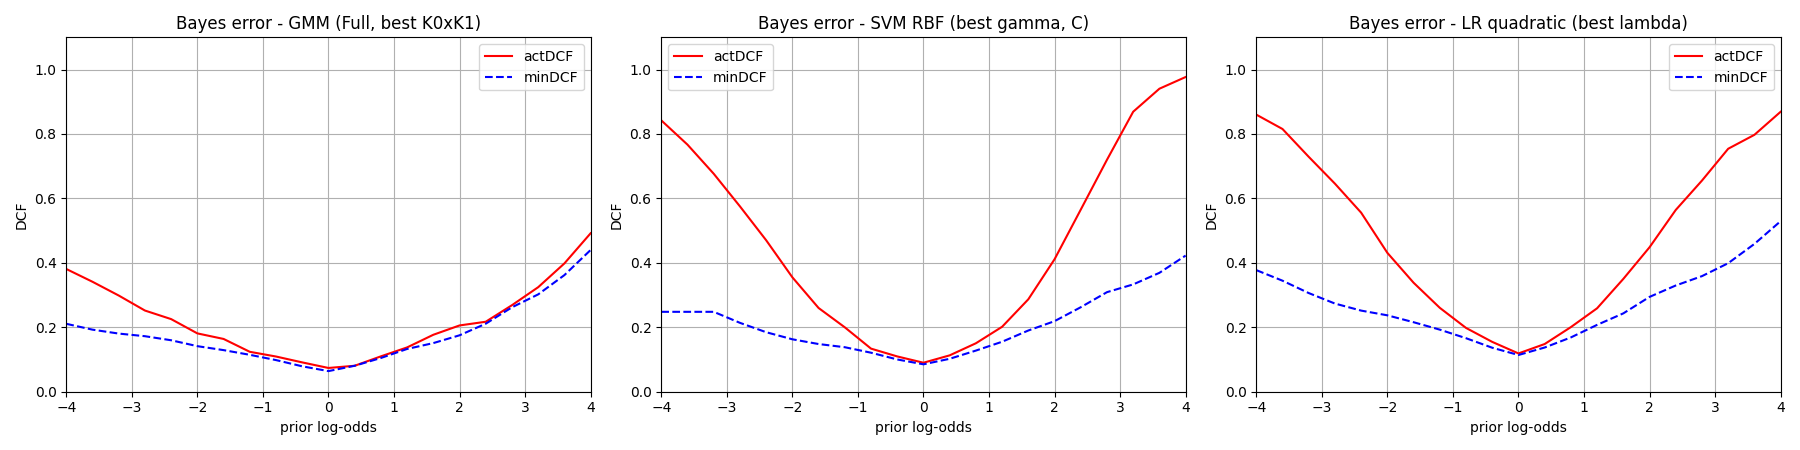
\includegraphics[width=\textwidth]{lab09_01_bayes_error_top3.png}
\caption{Bayes Error Plot for the top-3 best-of-family. (Left) GMM
         full: actDCF and minDCF very close over the whole region
         (well-calibrated). (Center) SVM RBF: actDCF $\gg$ minDCF in
         the tails (strong miscalibration). (Right) LR Quadratic:
         intermediate behavior.}
\end{figure}

\subsection{Answers to the Lab 9 project questions}

\begin{itemize}
\item \textbf{Which $K_0 \times K_1$ combinations work best?}
      Dominant pattern: increasing $K_1$ (components for the genuine
      class) improves minDCF up to $K_1=16$. Increasing $K_0$ has a
      modest, non-monotone benefit. The best is $K_0=1, K_1=16$
      (full-cov): consistent with the dataset structure observed in
      \S\ref{sec:lab2}. The fake class is essentially uni-modal
      $\rightarrow$ 1 Gaussian is enough. The genuine class is
      multi-modal (4 clusters on features 5--6) $\rightarrow$ many
      components are needed.

\item \textbf{Surprising results?} Yes: one might have expected a
      symmetric $K$ (e.g.\ $8\times 8$ or $16\times 16$). Instead the
      \textbf{asymmetric model} wins, reflecting the intrinsic
      complexity of the two classes.

\item \textbf{Comparison across methods (best per family):} GMM wins
      in minDCF (0.150 full / 0.132 diag), SVM RBF second (0.173),
      LR quadratic third (0.244), Gaussian baseline further
      (MVG $\approx 0.263$).

\item \textbf{Most promising model: GMM.} It combines:
      (a) better separability (lower minDCF);
      (b) better intrinsic calibration (actDCF close to minDCF),
      because GMM is generative and its LLR is a true ML density
      ratio.

\item \textbf{Consistent actDCF ranking?} No: SVM has much worse
      actDCF than GMM in the tails (factor $2+$); SVM should be
      \textbf{calibrated} for real-world applications.
\end{itemize}

%-----------------------------------------------------------------------------
\section{General discussion and conclusions}\label{sec:conclusions}
%-----------------------------------------------------------------------------

\subsection{Summary of design choices}

\textbf{Conventions adopted:}
\begin{itemize}
\item Samples are \textbf{columns} of $D \in \mathbb{R}^{M \times N}$
      with $M=6, N=6000$.
\item Class 1 (genuine) on top of the ratio:
      $\textrm{LLR} = \log p(x|1) - \log p(x|0)$.
\item Deterministic split (seed$=0$): 4000 training, 2000 validation.
\item ML estimate always on DTR; transformations (PCA, LDA)
      \textbf{never} estimated on DVAL.
\item Normalized DCF, theoretical threshold
      $t = -\log(\pi_T/(1-\pi_T))$ for actDCF.
\item Plots in PNG; text logs mirrored to terminal and file via
      \texttt{utils/logger.py}.
\end{itemize}

\subsection{Cross-lab comparison: model ranking (minDCF at $\tilde{\pi}=0.1$)}

\begin{table}[H]
\centering
\small
\begin{tabular}{rlrl}
\toprule
Rank & Model                                  & minDCF             & Characteristics \\
\midrule
1    & \textbf{GMM Diagonal ($8\times 16$)}    & \textbf{0.1324}    & Non-parametric, generative, well-calibrated \\
2    & GMM Full ($1\times 16$)                 & 0.1495             & Non-parametric, generative, well-calibrated \\
3    & SVM RBF ($\gamma=e^{-2}, C=32$)         & 0.1725             & Non-parametric, discriminative, miscalibrated \\
4    & SVM Poly $d=4$ (opt)                    & 0.1767             & Polynomial discriminative, miscalibrated \\
5    & LR Quadratic ($\lambda=3.2\cdot 10^{-2}$)& 0.2436            & Parametric quadratic discriminative \\
6    & SVM Poly $d=2$                          & 0.2455             & Quadratic discriminative, miscalibrated \\
7    & Naive Bayes Gaussian                    & 0.2570             & Parametric generative, diagonal \\
8    & MVG Full                                & 0.2629             & Parametric generative, full-cov \\
9    & Tied Gaussian                           & 0.3628             & Parametric generative, linear boundary \\
10   & LR linear / SVM linear                  & $\approx 0.36$     & Linear discriminative \\
\bottomrule
\end{tabular}
\end{table}

\subsection{Take-aways for an exam}

\begin{enumerate}
\item \textbf{The Lab 2 exploratory analysis already predicts the
      winner.} The 4 clusters on features 5--6 and the bimodality of
      the genuine class on those same features justify why a GMM with
      many components for genuine wins.

\item \textbf{Different model families have orthogonal strengths:}
      \begin{itemize}
      \item \emph{Parametric generative} (MVG, Naive, Tied): fast,
            output naturally calibrated as LLR, but Gaussian
            assumption fails on features 5--6.
      \item \emph{Parametric discriminative} (LR): output calibrated
            as log-posterior; with feature expansion (quadratic) it
            recovers MVG in expressiveness and sometimes beats it.
      \item \emph{Non-parametric discriminative} (kernel SVM): maximum
            boundary flexibility, but non-probabilistic output
            $\rightarrow$ calibration needed.
      \item \emph{Non-parametric generative} (GMM): combines
            flexibility and automatic calibration, the sweet spot for
            this task.
      \end{itemize}

\item \textbf{Relationship between models:}
      \begin{itemize}
      \item Tied Gaussian $\approx$ LDA $\approx$ Linear LR
            $\approx$ Linear SVM: all produce a linear boundary.
            They differ only in the training criterion.
      \item MVG $\approx$ Quadratic LR $\approx$ Poly $d=2$ SVM:
            all quadratic boundary.
      \item $K$-component GMM $\approx$ kernel SVM with RBF: both
            model non-parametric boundaries.
      \end{itemize}

\item \textbf{Calibration vs separability (minDCF vs actDCF):}
      \begin{itemize}
      \item \textbf{minDCF} measures the intrinsic quality of the
            sample \emph{ranking}.
      \item \textbf{actDCF} measures the quality of the
            \emph{decisions} based on the theoretical threshold.
      \item A model with low minDCF but high actDCF is one that ``can''
            classify but ``cannot'' decide $\rightarrow$
            \textbf{calibration} is required.
      \item Generative models (MVG, GMM) are usually better calibrated
            than discriminative ones (LR, especially SVM).
      \end{itemize}

\item \textbf{PCA does not always help.} On this task it does not
      improve Gaussian models and even slightly worsens Naive Bayes
      (introduces correlation in the new features). PCA is useful
      mainly when: (a) we have high dimensionality with noise;
      (b) we want to visualize. Not the case here.

\item \textbf{Regularization and dataset size:}
      \begin{itemize}
      \item Full DTR (4000 samples, 7 LR-linear parameters):
            regularization irrelevant.
      \item Reduced DTR (80 samples): regularization critical,
            classic bias/variance U-shape.
      \item Full DTR + Quadratic LR (42 parameters): regularization
            useful again (sample/parameter ratio drops to $\sim 95$).
      \end{itemize}
\end{enumerate}

\subsection{A natural extension: score calibration}

For this project, models have been saved to disk (see
\texttt{out/lab07/}, \texttt{out/lab08/},
\texttt{out/lab09/gmm\_full\_best\_llr.npy}) precisely to be used in a
future \textbf{calibration} lab. The flow would be:
\begin{enumerate}
\item Take the scores of an uncalibrated discriminative model
      (e.g.\ SVM RBF).
\item Fit a linear LR (\texttt{trainWeightedLogRegBinary} with target
      $\pi_T$) on the scores of a calibration subset.
\item Apply the affine transformation to the evaluation scores.
\item Compare actDCF before/after: we expect it to approach minDCF.
\end{enumerate}

\subsection{Possible future improvements (not implemented)}

\begin{itemize}
\item \textbf{Score-level fusion:} combine LR quadratic + GMM +
      SVM RBF via averaging or a multi-input calibrator.
\item \textbf{More aggressive cross-validation} for hyper-parameter
      selection.
\item \textbf{Z-normalization} of features before SVM.
\item \textbf{PCA pre-processing for regularized LR}.
\item \textbf{Tied-cov GMM} (shared covariances across components
      within the same class), not yet benchmarked as best-of-family.
\end{itemize}

%-----------------------------------------------------------------------------
\appendix
\section{PDF Lab \texorpdfstring{$\rightarrow$}{->} Script
          \texorpdfstring{$\rightarrow$}{->} Output mapping}
%-----------------------------------------------------------------------------

\begin{table}[H]
\centering
\scriptsize
\renewcommand{\arraystretch}{1.15}
\begin{tabularx}{\textwidth}{rLLLL}
\toprule
Lab & PDF & Script & Text log & Plot dir \\
\midrule
2 & \code{Iris\_Dataset.pdf}                  & \code{lab02\_iris\_dataset.py}              & \code{lab02\_iris\_dataset.txt}              & \code{plots/lab02/} \\
3 & \code{Dimensionality\_Reduction.pdf}      & \code{lab03\_dimensionality\_reduction.py}  & \code{lab03\_dimensionality\_reduction.txt}  & \code{plots/lab03/} \\
4 & \code{Probability\_Density\_Estimation.pdf} & \code{lab04\_density\_estimation.py}      & \code{lab04\_density\_estimation.txt}        & \code{plots/lab04/} \\
5 & \code{Generative\_Gaussian\_Models.pdf}    & \code{lab05\_gaussian\_classification.py}  & \code{lab05\_gaussian\_classification.txt}   & --- \\
6 & \code{BayesDecisionsModelEvaluation.pdf}  & \code{lab06\_bayes\_evaluation.py}          & \code{lab06\_bayes\_evaluation.txt}          & \code{plots/lab06/} \\
7 & \code{LogisticRegression.pdf}             & \code{lab07\_logistic\_regression.py}       & \code{lab07\_logistic\_regression.txt}       & \code{plots/lab07/} \\
8 & \code{SVM.pdf}                            & \code{lab08\_svm.py}                        & \code{lab08\_svm.txt}                        & \code{plots/lab08/} \\
9 & \code{GMM.pdf}                            & \code{lab09\_gmm.py}                        & \code{lab09\_gmm.txt}                        & \code{plots/lab09/} \\
\bottomrule
\end{tabularx}
\end{table}

%-----------------------------------------------------------------------------
\section{Models and hyper-parameters used}
%-----------------------------------------------------------------------------

\begin{table}[H]
\centering
\footnotesize
\begin{tabularx}{\textwidth}{lLLL}
\toprule
Model         & Parameters                                       & Hyper-param           & Best value \\
\midrule
MVG           & $\mu_c$ (6$\times$1), $\Sigma_c$ (6$\times$6) per $c\in\{0,1\}$ & ---            & --- \\
Naive         & as MVG but $\textrm{diag}(\Sigma_c)$            & ---                  & --- \\
Tied          & $\mu_c$ $+$ global $\Sigma$                     & ---                  & --- \\
PCA           & projection matrix (6$\times$m)                  & $m\in\{1..6\}$        & $m=6$ (no PCA) \\
LDA           & 1-D direction                                   & threshold            & mean-of-means or sweep \\
Linear LR     & $w$ (6), $b$ (1)                                & $\lambda$             & $10^{-2}$ (full), $10$ (reduced) \\
Weighted LR   & $w$, $b$                                        & $\lambda, \pi_T$       & $\pi_T=0.1, \lambda=32$ \\
Quadratic LR  & $w$ (42), $b$                                   & $\lambda$             & $3.2\cdot 10^{-2}$ \\
Linear SVM    & $w$, $b$                                        & $C, K$                & $C=0.32, K=1$ \\
Poly SVM      & $\alpha$ (4000)                                 & $C, d, c, \xi$        & $C=3.2\cdot 10^{-2}, d=2, c=1, \xi=0$ \\
RBF SVM       & $\alpha$ (4000)                                 & $C, \gamma, \xi$      & $C=32, \gamma=e^{-2}=0.135, \xi=1$ \\
GMM Full      & $(w_g, \mu_g, \Sigma_g)$ per $g, c$              & $K_0, K_1, \psi, \alpha_{\textrm{LBG}}$ & $K_0=1, K_1=16, \psi=10^{-2}, \alpha=0.1$ \\
GMM Diagonal  & as Full but $\textrm{diag}(\Sigma_g)$            & as Full              & $K_0=8, K_1=16$ \\
\bottomrule
\end{tabularx}
\end{table}

%-----------------------------------------------------------------------------
\section{Commands to reproduce the results}
%-----------------------------------------------------------------------------

\begin{Verbatim}[fontsize=\small, frame=single]
# Environment activation
source /home/nikcian/workspace/MPLR_Course/.venv/bin/activate
cd /home/nikcian/workspace/MPLR_Course/Project

# Run all labs sequentially
python experiments/lab02_iris_dataset.py
python experiments/lab03_dimensionality_reduction.py
python experiments/lab04_density_estimation.py
python experiments/lab05_gaussian_classification.py
python experiments/lab06_bayes_evaluation.py
python experiments/lab07_logistic_regression.py
python experiments/lab08_svm.py       # ~5-10 min for kernel SVMs
python experiments/lab09_gmm.py       # ~3-5 min for the 5x5 grid
\end{Verbatim}

All scripts accept an optional argument for the dataset, default $=$
\texttt{data/trainData.txt}.

\end{document}
